%\chapter{Aprendizado de Redes Bayesianas}
Muitas vezes, quando queremos construir uma \gls{bn}, o conhecimento do relacionamento de causa entre as variáveis do nosso dominio pode ser incerto, o custo de um especialista muito elevado, e principalmente, precisar as probabilidades dos de cada nó dados seus pode ser inviável. No entanto, se tivermos dados sobre o problema, isto pode facilitar muito esse processo de criação da \gls{bn}, tudo que precisamos fazer é adaptar técnicas de aprendizado de máquina para o escopo de \glspl{bn}. Pensando nisto o interesse em desenvolver e implementar estas técnicas vem aumentando nos últimos anos.

É importante observar que as probabilidades representadas por \gls{bn} pode ser Bayesiana ou Física. Quando construímos uma \gls{bn} a partir de conhecimento prévio tão somente, as probabilidades serão Bayesianas. No entanto se aprendermos estas estruturas a partir de dados, estas probabilidades serão físicas \cite{heck95}.

O aprendizado de uma \gls{bn} é dividido em duas etapas distintas e independentes
\begin{itemize}
	\item O Aprendizado da Estrutura da rede. Isto é, quais as relações de causas entre as variáveis do nosso domínio.
	\item O Aprendizado dos Parâmetros da rede. Isto é, dada a estrutura da rede, quais as probabilidades de cada um dos nós.
\end{itemize}

Obviamente para se aprender os parâmetros de uma rede é necessário que já se tenha a estrutura da pronta. Esta estrutura pode ter sido construída por um especialista, ou aprendida pelos dados. Entretanto o aprendizado de parâmetro é trivial de ser feito e por este motivo já se tornou uma tradição entre as publicações sobre de Aprendizado de Redes Bayesianas apresentar a aprendizagem de parâmetros antes da aprendizagem de estrutura. Nós também seguiremos esta tradição.

\section{Aprendizado de Parâmetros}
O aprendizado de parâmetros nada mais que encontrar a distribuição de probabilidade conjunta de cada variável aleatória presente na reade, representadas por \glspl{cpt}, dada a topologia da rede.

Seja $\textbf{X} = {X_1,X_2,...,X_n}$ para o conjunto de variáveis aleatórias do model, $B(S)$ para a estrutura da \gls{bn} e $\theta_s$ para os parâmetros da \gls{bn}. Pearl \cite{pearl88} provou que a função de distribuição conjunta de $\textbf{X}$ pode ser obitida como o produto das distribuições de probabilidades condicionais da variável da \gls{bn}, dado os seus pais. A partir da \autoref{eq:pearl} temos que:
\begin{equation}
	P(\textbf{X}|\theta_s, B(S)) = \prod_{i=1}^{n}p(x_i|pa_i,\theta_i,B(S))
\end{equation}
Onde $\theta_i$ é o vetor de prâmetros para $P(x_i|pa_i, \theta_i, B(S))$, $\theta_s$ é o vetor de parâmetros de $(\theta_1,...,\theta_n)$. O que desejamos é econtrar os parâmetros $\theta_s$ dado um conjunto de treinamento $D$ e a estrutura $B(S)$. Para isto avaliamos a expressão $P(\theta_s| D,B(S))$. É importante notar que $D$ deve ser um conjunto de terinamento completo e é respresentado por ${x_1,x_2,...,x_n}$, onde cada $x_i$ representa um caso do conjunto de dados observados. As incertezas são codificadas sobre os parâmetros $\theta_s$ por uma variável aleatória $\Theta_s$ e a função a priori $P(\theta_s|B(S))$. A função $P(x_i|pa_i,\theta_i,B(S))$ é vista como a função de distribuição local.

\iffalse
	Assumindo que se trata de dados discretos a função de distribuição local será dada por:
	\begin{equation}
	p(x_{i}^{k}|pa_{i}^{j},\theta_i, B(S)) = \theta_{ijk} > 0
	\end{equation}
	onde $pa_{i}^1,...,pa_{i}^{q_i}$são as $q_i$ instâncias possíveis dos pais de $x_i$, $\theta_i=((\theta_{ijk})_{k=1}^{r_i})_{j=1}^{q_i}$ e $\theta_{ijk}$ é a probabilidade de ocorrência do k-ésimo valor de $x_i$, dada a j-ésima configuração de pais de $x_i$, o vetor de parâmetros $\theta_i$ dessa distribuição de probabilidades e a estrutura $B(S)$.
\fi

A partir de manipulações aritméticas que fogem do escopo deste trabalho chegamos na seguinte equação:
\begin{equation}
P(X_i=x_i^k|Pais = pa_i^j) = \frac{\alpha_{ijk}+N_{ijk}}{\sum_{i}^{r_i}\alpha_{ijk}+N_{ij}}
\label{eq:param_learn}
\end{equation}

Seja o domínio de $X_i$ denotado por $D_{x_i}$
\begin{itemize}
	\item $X_i$ é a i-ésima variável da rede bayesiana;
	\item $x_i^k \in D_{x_i}$ é a k-ésima instância da variável $X_i$;
	\item $pa_i^j$ é a j-ésima instância da variável $X_i$;
	\item $\alpha_{ijk}$ é o parâmetro da distribuição de Dirichlet;
	\item $r_i$ é a cardinalidade dos estados da variável $X_i$, de $D_{x_i}$;
	\item $N_{ij}$ é o número total de ocorrências de $X_i$ dados os seus pais; $pa_i^j$, isto é, $N_{ij}=\sum_{k=1}^{n}N_{ijk}$
\end{itemize}

Os parâmetros $\alpha_{ijk}$ podem ser substituídos por 1, pois corresponde ao valor esperado da frequência de cada estado, admitindo-se uma distribuição uniforme para os estados de $X_i$, visto que, a princípio, não se tem nenhuma informação que permita estimação melhor para essa distribuição de probabilidades.

A seguir daremos um exemplo da aplicação dessa fórmula para o aprendizado da rede Ásia \ref{fig:red_asia} proposto por Lauritzen e Spielgelhater \cite{lauritzen88}. A tabela com os dados foi retirada de \cite{custodio05}


\begin{figure}[ht]
	\centering
	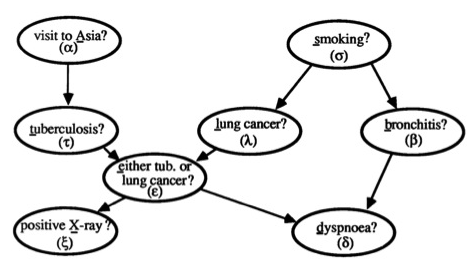
\includegraphics{figuras/red_asia}
	\caption[Rede Ásia]{Rede Ásia}
	\label{fig:red_asia}
\end{figure}

\begin{figure}[ht]
	\centering
	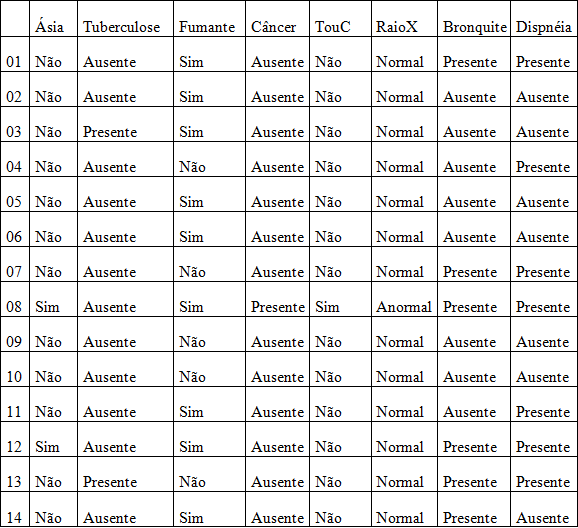
\includegraphics{figuras/tabela_asia}
	\caption[Dados para Treinamento para a rede Ásia]{Exemplo de conjunto de treinamento para a Rede Ásia}
	\label{fig:tabela_asia}
\end{figure}

\newtheorem{exmp}{Exemplo}[chapter]
\begin{exmp}
	Neste exemplo desejamos aprender os parâmetros para a variável dispnéia da rede Àsia, a partir do conjunto de treinamento apresentado na Tabela \ref{fig:tabela_asia}
\end{exmp}


Os pais da variável da variável Dispneia são TouC (coluna 4) e Bronquite (coluna 6), portanto $pa_7=[4,6]$. Os estados de TouC e Bronquite são, respectivamente representados por:
\begin{itemize}
	\item $D_x[4]=[0,1]$, onde 0 representa 'Não' e 1 'Sim'; 
	\item $D_x[6]=[0,1]$, onde 0 representa 'Ausente' e 1 representa 'Presente'.
\end{itemize} 
As possíveis instâncias para Dispneia são: $pa_7 = [[0,0]^0, [0,1]^1,[1,0]^2,[1,1]^3]$ onde por exemplo a instância 2: $[1,0]^2$ representa TouC assumindo o valor 'Sim ' e Bronquite assumindo o valor 'Ausente'.

A matriz $N_{ijk}$ para dispnéia, obtida através da contagem na matriz D das ocorrências de Dispneia, condicionadas as instâncias possíveis para os pais TouC e Bronquite, está apresentada na \refTab{tab:disp}

\tabela{Matriz $N_{ijk}$ Para Dispneia com Pais T ou C e Bronquite}{tab:disp}{| c | c | c | c | c |}%
{\hline
	& \multicolumn{4}{|c|}{Instancia dos Pais} \\\hline
	Dispneia & 0 & 1 & 2 & 3 \\\hline
	0 & 3 & 2 & 1 & 0 \\\hline
	1 & 1 & 7 & 0 & 0 \\\hline
	}%
A partir dessa taela é possível calcular a probabilidade associada a cada parâmetro da distribuição de probabilidade da variável aleatória DIspneia. A tabela de probabiliades condicionais de Dispneia, calculada com a \ref{eq:param_learn}, está representada na \refTab{tab:cpt_disp}

\tabela{CPT calculada para Dispneia}{tab:cpt_disp}{| c | c | c | c | c | c |}%
{\hline
	& TouC & 0 & 0 & 0 & 1 \\\hline
	& Bronquite & 0 & 1 & 0 & 1\\\hline\rule[-2.5ex]{0pt}{7ex}
	\multirow{2}{*}{Dispneia} & Sim & $\frac{1+3}{2+4} = 0.67$ & $\frac{1+2}{2+9} = 0.27$ & $\frac{1+1}{2+1} = 0.67$ & $\frac{1+0}{2+0} = 0.5$ \\\cline{2-6}\rule[-2.5ex]{0pt}{7ex}
	& Não & $\frac{1+1}{2+4}=0.33$ & $\frac{1+7}{2+9}=0.73$ & $\frac{1+0}{2+1}=0.33$ & $\frac{1+0}{2+0}=0.5$\\\hline
	
	
	
}%

\section{Aprendizado de Estrutura}
O Objetivo da aprendizagem da Estrutura é encontrar a topologia da \gls{bn} que mais se adéqua aos nossos dados. Para isto podemos atacar o problema de duas formas distintas:
\begin{itemize}
	\item Busca e pontuação: fazemos uma busca no conjunto de todos \gls{dag} existentes entre nossas variáveis usando heurísticas robustas o suficiente.
	\item Análise de dependência: utilizamos técnicas estatísticas bem desenvolvidas para analisar a dependência entre nossos dados e a partir deles inferir a estrutura da rede.
\end{itemize}

Vamos começar discutindo sobre algoritmos de busca e pontuação, apresentamos as heurísticas mais famosas.

\subsection{Busca e Pontuação}



\subsection{Análise de Dependência}

\section{Aprendizado Incremental}